\chapter{Électrons dans le potentiel cristallin}
	\section{Les électrons et les trous dans les semi-conducteurs}
	Un semi-conducteurs est un isolant dont la dernière bande remplie (bande 
	de valence) est peu séparée de la prochaine bande vide (bande de conduction)
	: cette distance est le \textit{gap}. \\
	Si ce gap n'est pas abusé, les électrons de la bande de valence peuvent être 
	excités thermiquement dans la bande de conduction, contribuant à la 
	conductivité du cristal. Mais, ces électrons partis laissent des états vides, 
	des \textit{trous} qui contribuent aussi à la conductivité.\\
	Un mécanisme analogue est la photoconductivité : on envoie des photons 
	d'énergie $\hbar\omega > \epsilon_G$ où $\epsilon_G$ est l'énergie du gap. 
	Cela crée des paires électrons-trous contribuant à la conductivité.\\
	
	\begin{wrapfigure}[7]{r}{3.5cm}
	\vspace{-0.8cm}
	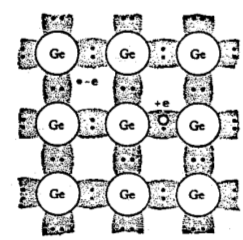
\includegraphics[scale=0.4]{ch8/image1.png}
	\captionof{figure}{ }
	\end{wrapfigure}
	Considérons les liaisons de valence dans un cristal. L'excitation d'un 
	électrons de la bande de valence à la bande de conduction est équivalente 
	à la rupture d'un lien de valence : l'électron est éjecté et devient 
	un porteur de charge libre. Le trou est le lien rompu auquel on peut 
	associer une charge positive\footnote{Car compensation des charges avant 
	son départ.}. Or ce trou peut se propager de proche en proche se comporter 
	comme un porteur de charge positive. 
	
		\subsection{Structure de bande}
		Les bandes de conductions possèdent plusieurs minima équivalents que l'on 
		nomme \textit{vallées}. Pour le Ge, ces minimas se trouvent sur le long des 
		direction (111) dans l'espace réciproque, soit exactement sur les limites 
		de zones.
		\begin{center}
		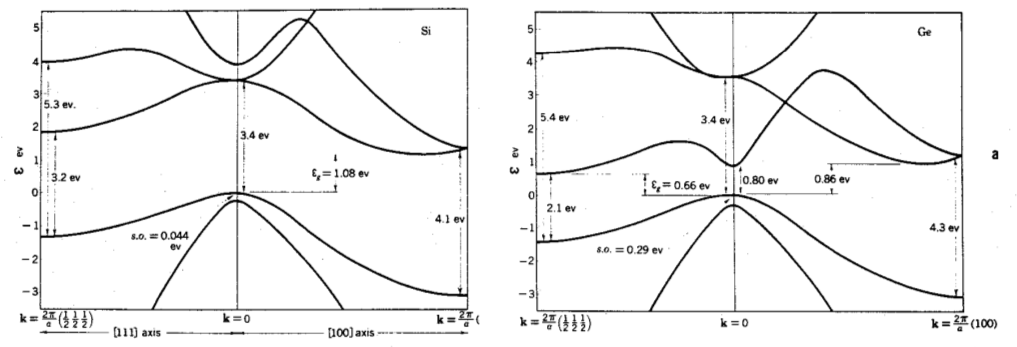
\includegraphics[scale=0.4]{ch8/image2.png}
		\captionof{figure}{ }
		\end{center}				
		Sur la partie gauche de l'image ci-dessus, nous avons un gap de 1.08 eV. 
		Il s'agit d'un gap \textit{indirect}, car la position du minimum d'énergie 
		de la bande de conduction n'est pas au même endroit que le maximum de la 
		bande de valence.
		Le gap sera ainsi \textit{direct} si la position des extremums est la même 
		pour la bande de valence et de conduction.
		Cette disposition influe grandement sur les propriétés optiques : pour avoir 
		une transition optique (au minimum 1.08 eV), on a besoin de la médiation 
		d'un phonon.\\
		On peut observer différent types de courbures. Si la courbure est faible, 
		la masse effective de trou sera grande et inversement. On parlera de 
		trou \textit{léger} et \textit{lourds}. Pour ceux qui ne l'ont pas vu, le 
		minimum se trouve légèrement à gauche de $b$.\\
		
		Autours des minimas se trouvent des zones isoénergétiques, décrites par des 
		ellipsoïdes de révolution. Plus tard, nous allons essayer de changer ces 
		ellipsoïdes en sphères pour se ramener au modèle de Sommerfeld.
		
	\section{Les centres donneurs et accepteurs dans les semiconducteurs}
		\subsection{Le silicium, quel homme}
		Le silicium pur c'est joli, mais pas super utile. Pour le rendre utile, 
		il faut le doper. Le \textit{dopage}, c'est introduire délibérément des 
		impuretés pour modifier le comportement de conductivité électrique des 
		semiconducteurs : impureté accepteur et donneur.\\
		
		Le Si est tétravalent (colonne 4 du tableau). Pour satisfaire ses liaisons 
		covalentes, il a quatre plus proches voisins (hybridation sp3) donnant lieu 
		à une gigantesque molécule covalente : c'est le cas du Si pur. Si l'on 
		rajoute des impuretés de valence cinq ou trois, par exemple de l'arsenic, 
		on va "remplacer" des atomes de Si par de l'As. Lors de l'élévation de la 
		température, cet électron supplémentaire ajouté (ou le défaut) va se détacher 
		et trouver de l'espace dans les bandes de conduction !
		
		\subsection{Impuretés dans le Si et le Ge}
		On vient de le voir, les impuretés peuvent affecter les propriétés électriques. 
		Étudions l'effet des impuretés dans le Si et le Ge. Si on ajoute un atome 
		d'impureté du groupe $V_B$ (phosphore, arsenic, antimoine) à la place d'un atome
		normal (avec le minimum de perturbation), un électron de valence provenant de 
		l'impureté restera en surnombre. Ces atomes d'impuretés qui peuvent s'ioniser 
		et abandonner un $e^-$ sont des \textit{donneurs}\footnote{Le cristal reste 
		naturellement neutre}.
		\begin{center}
		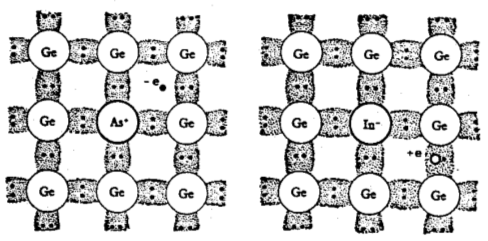
\includegraphics[scale=0.4]{ch8/image3.png}
		\captionof{figure}{A gauche un  électron du à l'impureté électrique. A droite, 
		un défaut d'électron autour de l'atome d'indium qui peut se balader et former un 
		trou}
		\end{center}						
		\newpage
		
		Cet électron en excès se déplace dans le potentiel coulombien $e/4\pi\epsilon r$ 
		du à l'ion d'impureté où $\epsilon$ tient compte de la réduction de la force 
		de Coulomb entre les charges par suite de la polarisation électrique du milieu
		.\footnote{C'est-à-dire ?}\\
		
		On peut voir cet électron autour de l'impureté comme un système hydrogénoïde : 
		il suffit de modifier le rydberg et le rayon de Bohr pour obtenir son équation 
		de Schrödinger :
		\begin{equation}
		\left(-\dfrac{\hbar^2}{2m_e^*}\nabla^2 - \dfrac{e^2}{4\pi\epsilon r}\right)\Psi(
		\vec r)	=(\epsilon_d-\epsilon_c)\Psi(\vec r)
		\end{equation}
		où $m_e^*$ est la masse effective isotrope, incorporant l'effet de la périodicité 
		cristalline, $\epsilon_d$ est l'énergie de l'électron supplémentaire du centre 
		donneur et $\epsilon_c$ est l'énergie du fond de la bande de conduction.\footnote{
		On mesure l'énergie par rapport à $\epsilon_c$ car l'électron devient "libre" quand 
		il entre dans la bande de conduction. Si l'énergie des électrons est inférieur à 
		$\epsilon_c$, il s'agit d'un état lié (il faut fournir une énergie positive pour 
		ioniser un électron dans la bande de conduction))}. Notre énergie de liaison sera 
		donc modifiée.\\
		Pour un électron de l'hydrogène atomique, son énergie est 
		\begin{equation}
		\epsilon_{Hn} = -\dfrac{e^4}{m	32\pi^2\hbar^2n^2\epsilon_0^2} = -\dfrac{13.6\ eV
		}{n^2}
		\end{equation}
		En effectuant les changements nécessaire (masse effective, permittivité du vide, 
		\dots) on trouve 
		\begin{equation}
		\epsilon_d-\epsilon_c = -\dfrac{\epsilon_0^2}{\epsilon^2}\dfrac{m^*}{m}\dfrac{13.6
		}{n^2}\ eV
		\end{equation}
		Le niveau $\epsilon_d$ est donc à une petite distance sous la bande de conduction. 
		Notre rayon de Bohr modifié est dès lors
		\begin{equation}
		r_d = \dfrac{\epsilon m}{\epsilon_0m_e^*}n^2\times 0,52\ \AA
		\end{equation}
		
		D'autres impuretés, comme le bore, l'alluminum, le gallium et l'indium sont des 
		impuretés trivalentes classiques que l'on nomme \textit{accepteurs} car elles 
		enlèvent des électrons aux bandes de valence, laissant des trous à leurs place.
		Pour ioniser un accepteur, il faut élever l'énergie d'un électron pour le faire 
		monter vers l'accepteur puis amener le trou dans la bande de valence. L'équation 
		de Schrödinger s'écrit alors
		\begin{equation}
		\left(-\dfrac{\hbar^2}{2m_e^*}\nabla^2 - \dfrac{e^2}{4\pi\epsilon r}\right)\Psi(
		\vec r)	=(\epsilon_v-\epsilon_a)\Psi(\vec r)		
		\end{equation}
		où $\epsilon_a$ est le niveau accepteur qui se place au-dessus du sommet $\epsilon_v$ 
		de la bande de valence et $(\epsilon_a-\epsilon_v)$ est l'énergie de liaison du trou 
		au centre accepteur localisé, chargé négativement.\\
		
		Alors qu'un électron descend en perdant de l'énergie, un trou monte. Sans impureté, 
		il y a autant d'électrons libres que de trous : le corps est dit \textit{intrinsèque}. 
		Si le nombre de donneurs est plus élevé que le nombre d'accepteur, l'ionisation 
		libèrera des électrons dans la bande de conduction : \textbf{type $n$} (excès d'électrons). 
		Si par contre il y a plus d'accepteurs, les trous seront libérés dans la bande de valence :
		de \textbf{type $p$} (défaut d'électrons).\\
		Comme on le verra en labo, le signe de la constante de Hall est un test grossier 
		pour déterminer le type.
		
		
		
		
		
		
		
		
		
		
		
		
		
		
		
		
		
		
		
		
		
		
		
		
		
		
		
		
		
		
		
